\begin{center}
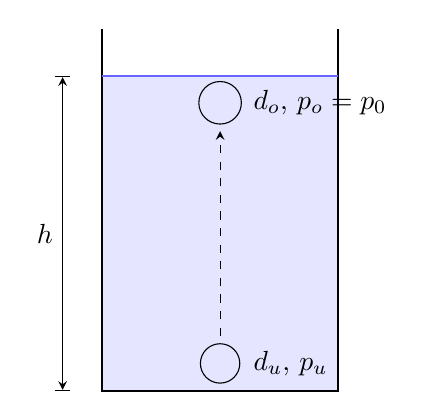
\begin{tikzpicture}[>=stealth]
 \fill[blue!10] (0,0) rectangle (3,4);
 \draw[thick] (0,4.6) -- (0,0) -- (3,0) -- (3,4.6);
 \draw[blue!60] (0,4) -- (3,4);
 \draw (1.5,0.35) circle (0.25);
 \node[right] at (1.8,0.35) {$d_\text{u}$, $p_\text{u}$};
 \draw (1.5,3.66) circle (0.27);
 \node[right] at (1.8,3.66) {$d_\text{o}$, $p_\text{o} = p_0$};
 \draw[->, dashed] (1.5,0.7) -- (1.5,3.3);
 \draw[|<->|] (-0.5,0) -- (-0.5,4) node[midway, left] {$h$};
\end{tikzpicture}
\end{center}

Die Temperatur und die Gasmenge in der Blase bleiben gleich. Am Boden herrscht zusätzlich zum Luftdruck der Schweredruck des Wassers. Mit dem Luftdruck $p_0 = \ncpo$ (Normaldruck) und der Dichte des Mineralwassers $\rho \approx \rW$ (wie Wasser, FoTaBe S.~192) ist
\begin{align}
 p_\text{u} &= \pUnF = \ncpo + \rW\cdot\gE\cdot\hgl = \pUn
\end{align}
Nach Boyle-Mariotte ist $p_\text{u}V_\text{u} = p_\text{o}V_\text{o}$, und das Volumen der Kugel ist proportional zu $d^3$:
\begin{align}
 \left(\frac{d_\text{o}}{d_\text{u}}\right)^3 &= \frac{V_\text{o}}{V_\text{u}} = \frac{p_\text{u}}{p_\text{o}}
\end{align}
Damit wird
\begin{align}
 \frac{d_\text{o}}{d_\text{u}} &= \dQoF = \sqrt[3]{\frac{\pUn}{\ncpo}} = \dQo
\end{align}
Der Durchmesser nimmt also zu um
\begin{align}
 \frac{\Delta d}{d_\text{u}} &= \ddrF = \ddr \approx \result{\ddrP{0}{2}}
\end{align}
In echtem Mineralwasser wächst die Blase zusätzlich, weil Kohlendioxid aus dem Wasser in die Blase diffundiert; dieser Effekt ist hier nicht berücksichtigt.
